%
\clearpage\onecolumn
\begingroup
\newcolumntype{B}{S[table-auto-round = true,exponent-product=\cdot,scientific-notation=true,table-figures-decimal=2,table-figures-integer=2,table-figures-exponent=1]}
\newcolumntype{T}{S[table-auto-round = true,table-format=2.2]}
% % \rotFPtop=0pt plus 1fil
% \rotFPtop=0pt
% \rotFPbot=0pt plus 1fil
\begin{sidewaystable}
\centering
% \begin{table}
\caption{Raw numbers for the comparison benchmarks. \emph{ops} is number of
  operations (higher is better), \emph{time (s)} is time in seconds (lower is
  better), \emph{ops / s} is number of operations per second (higher is better).}
% \begin{sideways}
\smaller\smaller\smaller
\sisetup{table-number-alignment = center}
% \hspace*{-1cm}
\begin{tabular}{%
c@{}r
B@{}T@{}B
B@{}T@{}B
B@{}T@{}B
B@{}T@{}B
B@{}T@{}B
B@{}T@{}B
B@{}T@{}B
}
\toprule
	&&\multicolumn{3}{c}{ContextL}&\multicolumn{3}{c}{ContextJS Edge}&\multicolumn{3}{c}{ContextJS Chrome OSX}&\multicolumn{3}{c}{ContextJS Chrome Win}&\multicolumn{3}{c}{ContextPy Python OSX}&\multicolumn{3}{c}{ContextPy PyPy OSX}&\multicolumn{3}{c}{ContextPyPy PyPy OSX} \\ 
\midrule
	&&{ops }&{ time (s) }&{ ops / s }&{ ops }&{ time (s) }&{ ops / s }&{ ops }&{ time (s) }&{ ops / s }&{ ops }&{ time (s) }&{ ops / s }&{ ops }&{ time (s) }&{ ops / s }&{ ops }&{ time (s) }&{ ops / s }&{ ops }&{ time (s) }& {ops / s} \\ 
\midrule
\parbox[t]{2mm}{\multirow{10}{*}{\rotatebox[origin=c]{90}{NoLayer}}}
	& 1 & 819200000 & 6.9630000000000001 & 117650438.02958494 & 838860800 & 7.7190000000000003 & 108674802.43554865 & 3355443200 & 9.5549999999999997 & 351171449.50287807 & 3355443200 & 9.8190000000000008 & 341729626.23485076 & 25600000 & 5.3390000000000004 & 4794905.4129986884 & 819200000 & 8.4580000000000002 & 96855048.47481674 & 819200000 & 8.3810000000000002 & 97744899.17670922 \\ 
	& 2 & 409600000 & 5.2130000000000001 & 78572798.77230002 & 838860800 & 8.2560000000000002 & 101606201.55038759 & 3355443200 & 9.6029999999999998 & 349416140.78933668 & 1677721600 & 5.1079999999999997 & 328449804.22866094 & 25600000 & 9.0579999999999998 & 2826230.9560609409 & 819200000 & 9.8049999999999997 & 83549209.586945444 & 409600000 & 5.0069999999999997 & 81805472.33872579 \\ 
	& 3 & 409600000 & 6.41 & 63900156.006240249 & 838860800 & 8.8960000000000008 & 94296402.87769784 & 3355443200 & 9.59 & 349889801.87695515 & 1677721600 & 5.335 & 314474526.71040303 & 12800000 & 6.0030000000000001 & 2132267.1997334664 & 409600000 & 5.2039999999999997 & 78708685.626441196 & 409600000 & 5.34 & 76704119.850187272 \\ 
	& 4 & 409600000 & 8.3510000000000009 & 49048018.201412998 & 419430400 & 5.7960000000000003 & 72365493.443754315 & 3355443200 & 9.5760000000000005 & 350401336.67502087 & 1677721600 & 5.19 & 323260423.89210016 & 12800000 & 7.64 & 1675392.6701570682 & 409600000 & 5.9710000000000001 & 68598224.752972707 & 409600000 & 6.0880000000000001 & 67279894.875164255 \\ 
	& 5 & 409600000 & 9.9830000000000005 & 41029750.575979166 & 419430400 & 5.327 & 78736699.831049368 & 3355443200 & 9.6199999999999992 & 348798669.43866944 & 1677721600 & 5.859 & 286349479.43335038 & 12800000 & 8.8979999999999997 & 1438525.5113508655 & 409600000 & 6.5860000000000003 & 62192529.608259946 & 409600000 & 6.7140000000000004 & 61006851.355376817 \\ 
	& 6 & 204800000 & 5.9749999999999996 & 34276150.627615064 & 419430400 & 9.7509999999999994 & 43014090.862475649 & 1677721600 & 5.2380000000000004 & 320298129.05689192 & 1677721600 & 6.6890000000000001 & 250817999.70100164 & 6400000 & 5.1790000000000003 & 1235759.7991890325 & 409600000 & 7.6550000000000002 & 53507511.430437624 & 409600000 & 7.7110000000000003 & 53118921.02191674 \\ 
	& 7 & 204800000 & 10.78 & 18998144.712430429 & 209715200 & 9.1310000000000002 & 22967385.828496329 & 1677721600 & 6.22 & 269730160.7717042 & 1677721600 & 8.9610000000000003 & 187224818.65863183 & 6400000 & 6.0289999999999999 & 1061535.9097694478 & 409600000 & 8.3409999999999993 & 49106821.72401391 & 409600000 & 8.2100000000000009 & 49890377.588306941 \\ 
	& 8 & 102400000 & 5.0149999999999997 & 20418743.76869392 & 209715200 & 8.1069999999999993 & 25868410.016035527 & 1677721600 & 6.9820000000000002 & 240292409.05184761 & 1677721600 & 9.3840000000000003 & 178785336.743393 & 6400000 & 6.5839999999999996 & 972053.46294046182 & 409600000 & 9.3879999999999999 & 43630166.169578187 & 409600000 & 9.516 & 43043295.502311893 \\ 
	& 9 & 102400000 & 6.2290000000000001 & 16439235.832396854 & 209715200 & 8.7490000000000006 & 23970190.878957592 & 1677721600 & 8.1199999999999992 & 206615960.59113303 & 838860800 & 5.8289999999999997 & 143911614.34208271 & 6400000 & 7.2430000000000003 & 883611.763081596 & 204800000 & 5.0979999999999999 & 40172616.712436251 & 204800000 & 5.133 & 39898694.720436394 \\ 
	& 10 & 102400000 & 6.1890000000000001 & 16545483.923089352 & 209715200 & 9.5370000000000008 & 21989640.348117854 & 1677721600 & 8.8940000000000001 & 188635214.75151786 & 838860800 & 6.8090000000000002 & 123198825.08444706 & 6400000 & 8.0510000000000002 & 794932.30654577073 & 204800000 & 5.3739999999999997 & 38109415.705247492 & 204800000 & 5.375 & 38102325.58139535 \\ 
	% {WithLayer} &  &  &  &  &  &  &  &  &  &  &  &  &  &  &  &  &  &  &  &  &  \\ 
\midrule
\parbox[t]{2mm}{\multirow{10}{*}{\rotatebox[origin=c]{90}{WithLayer}}}
	& 0 & 409600000 & 5.1829999999999998 & 79027590.198726609 & 409600 & 9.1379999999999999 & 44823.812650470565 & 3276800 & 7.0030000000000001 & 467913.75124946452 & 3276800 & 17.507000000000001 & 187170.84594733533 & 3200000 & 16.321999999999999 & 196054.40509741454 & 1638400000 & 5.5590000000000002 & 294729267.85393053 & 3276800000 & 8.0009999999999994 & 409548806.39920014 \\ 
	& 1 & 204800000 & 7.2610000000000001 & 28205481.338658586 & 819200 & 8.5749999999999993 & 95533.527696793011 & 1638400 & 5.0279999999999996 & 325855.21081941132 & 819200 & 8.1449999999999996 & 100577.04112952732 & 3200000 & 27.834 & 114967.30617230725 & 409600000 & 5.8230000000000004 & 70341748.239738956 & 1638400000 & 7.7 & 212779220.77922076 \\ 
	& 2 & 204800000 & 8.7430000000000003 & 23424453.84879332 & 409600 & 5.3460000000000001 & 76618.032173587722 & 1638400 & 6.335 & 258626.67719021311 & 409600 & 5.0010000000000003 & 81903.61927614476 & 3200000 & 39.341999999999999 & 81338.010268923797 & 204800000 & 5.0990000000000002 & 40164738.183957636 & 1638400000 & 9.7889999999999997 & 167371539.48309326 \\ 
	& 3 & 204800000 & 9.5429999999999993 & 21460756.575500369 & 409600 & 5.7640000000000002 & 71061.762664816095 & 1638400 & 7.4189999999999996 & 220838.38792290067 & 409600 & 6.0880000000000001 & 67279.89487516426 & 3200000 & 50.441000000000003 & 63440.45518526595 & 204800000 & 7.5490000000000004 & 27129421.11537952 & 819200000 & 6.0129999999999999 & 136238150.67354065 \\ 
	& 4 & 102400000 & 5.5579999999999998 & 18423893.486865781 & 409600 & 6.41 & 63900.15600624025 & 1638400 & 8.5779999999999994 & 191000.23315458151 & 819200 & 6.4870000000000001 & 126283.33590257438 & 3200000 & 61.743000000000002 & 51827.737557293942 & 102400000 & 5.9320000000000004 & 17262306.136210382 & 409600000 & 7.4359999999999999 & 55083378.160301238 \\ 
	& 5 & 102400000 & 6.2489999999999997 & 16386621.859497521 & 409600 & 7.6260000000000003 & 53710.988722790455 & 1638400 & 9.93 & 164994.96475327291 & 819200 & 7.1859999999999999 & 113999.44336209296 & 3200000 & 73.191000000000003 & 43721.222554685686 & 102400000 & 6.4960000000000004 & 15763546.798029555 & 409600000 & 8.1530000000000005 & 50239175.763522625 \\ 
	& 6 & 102400000 & 6.915 & 14808387.563268257 & 409600 & 8.141 & 50313.229333005773 & 819200 & 5.5250000000000004 & 148271.49321266968 & 819200 & 8.1159999999999997 & 100936.42188270084 & 3200000 & 84.168999999999997 & 38018.747995105085 & 102400000 & 7.7380000000000004 & 13233393.641767899 & 409600000 & 9.8659999999999997 & 41516318.670180418 \\ 
	& 7 & 102400000 & 11.725 & 8733475.4797441363 & 409600 & 8.6389999999999993 & 47412.895010996646 & 819200 & 6.12 & 133856.20915032679 & 819200 & 9.0399999999999991 & 90619.469026548686 & 3200000 & 95.977000000000004 & 33341.321358242079 & 51200000 & 9.7070000000000007 & 5274544.1434016684 & 51200000 & 7.048 & 7264472.190692395 \\ 
	& 8 & 51200000 & 6.2450000000000001 & 8198558.8470776621 & 409600 & 9.5530000000000008 & 42876.583272270487 & 819200 & 6.61 & 123933.43419062026 & 409600 & 5.2110000000000003 & 78602.955286893106 & 3200000 & 106.785 & 29966.755630472446 & 12800000 & 5.7930000000000001 & 2209563.2660107026 & 12800000 & 5.7720000000000002 & 2217602.2176022176 \\ 
	& 9 & 51200000 & 8.1649999999999991 & 6270667.4831598289 & 204800 & 5.2460000000000004 & 39039.268013724737 & 819200 & 7.2910000000000004 & 112357.70127554519 & 409600 & 5.375 & 76204.651162790702 & 3200000 & 119.71299999999999 & 26730.597345317554 & 12800000 & 7.2240000000000002 & 1771871.5393133997 & 12800000 & 7.0129999999999999 & 1825181.8052188794 \\ 
	% {Activation} &  &  &  &  &  &  &  &  &  &  &  &  &  &  &  &  &  &  &  &  &  \\ 
\midrule
\parbox[t]{2mm}{\multirow{6}{*}{\rotatebox[origin=c]{90}{Activation}}}
	& 0 & 102400000 & 5.6680000000000001 & 18066337.33239238 & 204800 & 9.8149999999999995 & 20866.021395822721 & 819200 & 9.0500000000000007 & 90519.337016574573 & 409600 & 8.7729999999999997 & 46688.703978114674 & 3200000 & 85.983000000000004 & 37216.659107032785 & 102400000 & 6.4829999999999997 & 15795156.563319452 & 409600000 & 7.6980000000000004 & 53208625.617043383 \\ 
	& 1 & 102400000 & 7.56 & 13544973.544973545 & 102400 & 5.36 & 19104.477611940296 & 409600 & 6.6609999999999996 & 61492.268428163945 & 204800 & 6.1669999999999998 & 33209.015728879524 & 3200000 & 96.156999999999996 & 33278.908451802781 & 102400000 & 6.2859999999999996 & 16290168.628698697 & 204800000 & 5.0979999999999999 & 40172616.712436251 \\ 
	& 2 & 102400000 & 8.5559999999999992 & 11968209.443665266 & 102400 & 7.306 & 14015.877361073091 & 409600 & 9.2970000000000006 & 44057.222760030112 & 204800 & 8.4339999999999993 & 24282.665401944512 & 3200000 & 105.76600000000001 & 30255.469621617533 & 102400000 & 9.5779999999999994 & 10691167.258300273 & 102400000 & 6.383 & 16042613.191289362 \\ 
	& 3 & 102400000 & 9.9130000000000003 & 10329869.867850298 & 102400 & 7.7039999999999997 & 13291.796469366564 & 204800 & 6.3550000000000004 & 32226.59323367427 & 102400 & 5.6829999999999998 & 18018.652120358965 & 3200000 & 117.35899999999999 & 27266.762668393563 & 12800000 & 6.4889999999999999 & 1972568.962860225 & 12800000 & 6.92 & 1849710.9826589595 \\ 
	& 4 & 25600000 & 6.2809999999999997 & 4075784.1108103809 & 102400 & 9.2479999999999993 & 11072.664359861592 & 204800 & 8.5869999999999997 & 23850.005822755327 & 102400 & 7.4589999999999996 & 13728.381820619386 & 3200000 & 128.37200000000001 & 24927.554295329195 & 12800000 & 6.9560000000000004 & 1840138.0103507761 & 12800000 & 7.3330000000000002 & 1745533.8879039956 \\ 
	& 5 & 51200000 & 11.465999999999999 & 4465375.8939473229 & 51200 & 5.4160000000000004 & 9453.4711964549479 & 102400 & 5.6340000000000003 & 18175.363862264821 & 102400 & 9.6430000000000007 & 10619.10193923053 & 3200000 & 140.78200000000001 & 22730.178573965419 & 12800000 & 7.4569999999999999 & 1716507.9790800591 & 12800000 & 7.8929999999999998 & 1621690.1051564678 \\ 
\bottomrule
\end{tabular}
% \end{sideways}
% \end{table}
\end{sidewaystable}
\endgroup
\clearpage

\begin{figure}
  \centering
  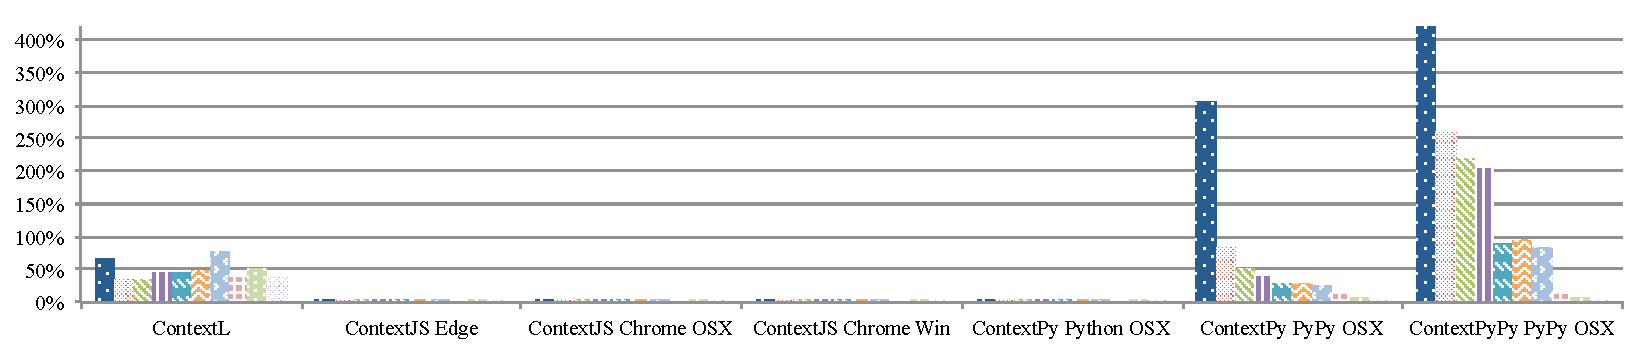
\includegraphics[width=\linewidth]{bench/malte-a/malte-a-1}
  \caption{Bench a overview}
  \label{fig:malte-a-overview}
\end{figure}

%%% Local Variables:
%%% mode: latex
%%% TeX-master: "cop2016-sidewayscomp"
%%% End:


\begingroup
\newcolumntype{P}{S[table-format=3.2]<{{\,\si{\percent}}}}
\begin{table*}
\centering
\caption{Bench A raw ratios}
\smaller
\begin{tabular}{rPPPPPPP}
\toprule
 & \multicolumn{1}{c}{ContextL} & \multicolumn{1}{c}{ContextJS} & \multicolumn{1}{c}{ContextJS} & \multicolumn{1}{c}{ContextJS} & \multicolumn{1}{c}{ContextPy} & \multicolumn{1}{c}{ContextPy} & \multicolumn{1}{c}{ContextPyPy}\\
 & \multicolumn{1}{c}{~} & \multicolumn{1}{c}{Edge} & \multicolumn{1}{c}{Chrome OSX} & \multicolumn{1}{c}{Chrome Win} & \multicolumn{1}{c}{Python OSX} & \multicolumn{1}{c}{PyPy OSX} & \multicolumn{1}{c}{PyPy OSX}\\
\midrule
no activate layer & 67.17 & 0.04 & 0.13 & 0.05 & 4.09 & 304.30 & 419.00 \\
1 active layer & 35.90 & 0.09 & 0.09 & 0.03 & 4.07 & 84.19 & 260.10 \\
2 active layer & 36.66 & 0.08 & 0.07 & 0.03 & 3.81 & 51.03 & 218.20 \\
3 active layer & 43.75 & 0.10 & 0.06 & 0.02 & 3.79 & 39.55 & 202.49 \\
4 active layer & 44.90 & 0.08 & 0.05 & 0.04 & 3.60 & 27.76 & 90.29 \\
5 active layer & 47.81 & 0.12 & 0.05 & 0.05 & 3.54 & 29.46 & 94.58 \\
6 active layer & 77.95 & 0.22 & 0.05 & 0.05 & 3.58 & 26.95 & 83.22 \\
7 active layer & 42.77 & 0.18 & 0.06 & 0.05 & 3.43 & 12.09 & 16.88 \\
8 active layer & 49.87 & 0.18 & 0.06 & 0.05 & 3.39 & 5.50 & 5.56 \\
9 active layer & 37.90 & 0.18 & 0.06 & 0.06 & 3.36 & 4.65 & 4.79 \\
\bottomrule
\end{tabular}
\end{table*}


\begin{table*}
\centering
\caption{Bench B raw ratios}
\smaller
\begin{tabular}{rPPPPPPP}
\toprule
 & \multicolumn{1}{c}{ContextL} & \multicolumn{1}{c}{ContextJS} & \multicolumn{1}{c}{ContextJS} & \multicolumn{1}{c}{ContextJS} & \multicolumn{1}{c}{ContextPy} & \multicolumn{1}{c}{ContextPy} & \multicolumn{1}{c}{ContextPyPy}\\
 & \multicolumn{1}{c}{~} & \multicolumn{1}{c}{Edge} & \multicolumn{1}{c}{Chrome OSX} & \multicolumn{1}{c}{Chrome Win} & \multicolumn{1}{c}{Python OSX} & \multicolumn{1}{c}{PyPy OSX} & \multicolumn{1}{c}{PyPy OSX}\\
\midrule
no activate layer&100.00&100.00&100.00&100.00&100.00&100.00&100.00 \\
1 active layer&74.97&91.56&50.00&71.13&89.42&103.13&75.50 \\
2 active layer&66.25&67.17&50.00&52.01&81.30&67.69&30.15 \\
3 active layer&57.18&63.70&25.00&38.59&73.26&12.49&3.48 \\
4 active layer&22.56&53.07&25.00&29.40&66.98&11.65&3.28 \\
5 active layer&24.72&45.31&12.50&22.74&61.08&10.87&3.05 \\
\bottomrule
\end{tabular}
\end{table*}
\endgroup
%%% Local Variables:
%%% mode: latex
%%% TeX-master: "cop2016-sidewayscomp"
%%% End:
